%%%%%%%%%%%%%%%%%%%%%%%%%%%%%%%%%%%%%%%%%
% University/School Laboratory Report
% LaTeX Template
% Version 3.1 (25/3/14)
%
% This template has been downloaded from:
% http://www.LaTeXTemplates.com
%
% Original author:
% Linux and Unix Users Group at Virginia Tech Wiki 
% (https://vtluug.org/wiki/Example_LaTeX_chem_lab_report)
%
% License:
% CC BY-NC-SA 3.0 (http://creativecommons.org/licenses/by-nc-sa/3.0/)
%
%%%%%%%%%%%%%%%%%%%%%%%%%%%%%%%%%%%%%%%%%

%----------------------------------------------------------------------------------------
%	PACKAGES AND DOCUMENT CONFIGURATIONS
%----------------------------------------------------------------------------------------

\documentclass{article}

\usepackage[version=3]{mhchem} % Package for chemical equation typesetting
\usepackage{siunitx} % Provides the \SI{}{} and \si{} command for typesetting SI units
\usepackage{graphicx} % Required for the inclusion of images
\usepackage{natbib} % Required to change bibliography style to APA
\usepackage{amsmath} % Required for some math elements 
\usepackage[utf8]{inputenc}
\usepackage[margin=1.2in]{geometry}

\setlength\parindent{0pt} % Removes all indentation from paragraphs

% \renewcommand{\labelenumi}{\alph{enumi}.} % Make numbering in the enumerate environment by letter rather than number (e.g. section 6)

\renewcommand{\figurename}{Figura}
\renewcommand{\tablename}{Tabla}
\renewcommand\refname{Referencias}

\def\mean#1{\left< #1 \right>}
%\usepackage{times} % Uncomment to use the Times New Roman font

%----------------------------------------------------------------------------------------
%	DOCUMENT INFORMATION
%----------------------------------------------------------------------------------------

\title{M\'etodos num\'ericos para la Ciencia e Ingenier\'ia \\ Tarea 6: Métodos Aleatorios} % Title

\author{Felipe Toledo Bittner} % Author name

\date{\today} % Date for the report

\begin{document}

\maketitle % Insert the title, author and date

%----------------------------------------------------------------------------------------
%	SECTION 1
%----------------------------------------------------------------------------------------

\section{Integración de Montecarlo}

\subsection{Introducción}
\label{sec:introduccion_P1}

Se desea obtener la posición del centro de masa de un sólido formado por la intersección de un toro con un cilindro, descrito por las ecuaciones (\ref{eq:toro}) y (\ref{eq:cilindro}).

\begin{equation}
  Toro:\ z^2 + \left( \sqrt{x^2 + y^2} - 3 \right)^2 \leq 1
  \label{eq:toro}
\end{equation}

\begin{equation}
  Cilindro:\ (x - 2)^2 + z^2 \leq 1
  \label{eq:cilindro}
\end{equation}

La densidad del sólido no es uniforme y es descrita por la fórmula (\ref{eq:densidad}). Debido a esto último, realizar una integración analítica para encontrar el centro de masa puede resultar complejo, por lo que se decide utilizar el método numérico de Monte Carlo para estimar su posición.

\begin{equation}
  \rho(x, y, z) = 0.5 (x^2 + y^2 + z^2)
  \label{eq:densidad}
\end{equation}

Las integrales que se deben calcular para obtener la coordenada $x^i$ del centro de masa son las siguientes:

\begin{equation}
  M = \int_V \rho(\vec{r}) dx dy dz \approx \sum_j \rho(\vec{r_j}) \Delta V
  \label{eq:calculo_masa}
\end{equation}

\begin{equation}
  T^i = \int_V x^i \rho(\vec{r}) dx dy dz \approx \sum_j x_j \rho(\vec{r_j}) \Delta V
  \label{eq:calculo_torque}
\end{equation}


En este caso $V$ es el volumen del cuerpo, condición que será relajada para el cálculo numérico y $\Delta V \approx \frac{V}{N}$, con $N$ la cantidad de términos en la suma. El cálculo de $x_i$ se realiza de la forma indicada en la ecuación (\ref{eq:error}). Como cada integral obtenida con el método de Monte Carlo posee un error asociado, este se propagará quedando $x^i = \mean{x^i} \pm \Delta x^i$.

\begin{equation}
  x^i = \frac{\mean{T^i} + \Delta T^i}{\mean{M} + \Delta M} = \frac{\mean{T^i}}{\mean{M}} \pm \frac{\mean{T^i}}{\mean{M}} \sqrt{ \left( \frac{\Delta T^i}{\mean{T^i}} \right)^2 + \left( \frac{\Delta M}{\mean{M}} \right)^2 }
  \label{eq:error}
\end{equation}

\subsection{Solución implementada}

Para usar el algoritmo de Monte Carlo, resulta útil definirse un volumen $W$ que contenga a $V$, pero posea una geometría mas sencilla. Para este caso se utilizará un $W$ con forma de caja rectangular que acote de forma lo más precisa posible al sólido en estudio.

En la Figura \ref{fig:interseccion_P1} se puede ver que el volumen del sólido está contenido en $ [-1 \le z \le 1]$ y $[1 \le x \le 3]$. Realizando un despeje sencillo en $x = 1$, $z = 0$ se pueden obtener los valores extremos de $y$, que son $y^* = \pm \sqrt{15}$. Como se realizan integrales sobre volumen, el error por la resolución de los números de punto flotante debiese resultar despreciable, por lo que se decide usar el intervalo $[-\sqrt{15} \le y \le \sqrt{15} ]$ para terminar de definir el volumen $W$.

\begin{figure}[ht]
  \centering
  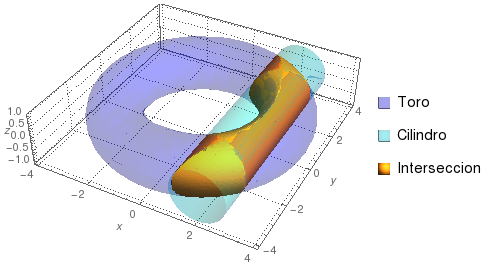
\includegraphics[scale = 0.5]{images/interseccion_P1.png}
  \caption{La figura naranja es el sólido en estudio. Está formado por el volumen que se obtiene al intersectar el toro (celeste) con el cilindro (azul) descritos en la Sección \ref{sec:introduccion_P1}. }
  \label{fig:interseccion_P1}
\end{figure}

En este volumen $W$ se usa el método de Monte Carlo, evaluando puntos generados al azar mediante una distribución uniforme, acotada por los intervalos correspondientes a cada coordenada. En caso de que un punto caiga fuera del sólido, se define $\rho = 0$ para anular su contribución a la integral.

\section{Resultados}

Realizando el cálculo con $N = 10^6$ se obtienen los valores de la Tabla \ref{tab:resultados}. Al comparar con la Figura \ref{fig:interseccion_P1} se observa que las coordenadas calculadas para el centro de masa están en el espacio ocupado por el sólido y parecen razonables.

\begin{table}[hl]
\centering
\begin{tabular}{|c|c|c|}
\hline
  Parámetro & Resultado \\
  \hline
  $M$ & $71.00 \pm 0.08$  \\ \hline
  $x_{CM}$ & $2.081 \pm 0.003$\\ \hline
  $y_{CM}$ & $0.001 \pm 0.003$\\ \hline
  $z_{CM}$ & $1 \cdot 10^{-4} \pm 7 \cdot 10^{-4}$\\ \hline
\end{tabular}
\caption{Tabla con resultados del cálculo numérico para la masa $M$ y las coordenadas del centro de masa $x^i_{CM}$.}
\label{tab:resultados}
\end{table}

\subsection{Caso 1}

En este caso se modela un sistema de Fisher-KPP, el cual consiste en la siguiente ecuación:

\begin{equation}
  \frac{\partial n}{\partial t} = \gamma \frac{\partial^2n}{\partial x^2} + \mu n - \mu n^2
  \label{Fisher-KPP}
\end{equation}

En este caso $n$ representa la densidad de una especie en función del tiempo y la posición. Los parámetros usados son:

\begin{enumerate}
  \item Largo de 1 [m]
  \item Discretizado de 500 puntos
  \item $\gamma$ = 0.001
  \item $\mu  = 1.5$
  \item Resolución: $h = 0.001$[s], $\Delta x = 0.002$[m]
  \item Condiciones de borde: $n(t, x=0) = 1$ y $n(t, x=1) = 0$
  \item Condiciones iniciales: $ n(0, x) = e^{-x^2/0.1} $
  \item Tiempo final de integración: $t_f = 4[s]$
\end{enumerate}

Tras integrar la ecuación para 4 segundos, se obtienen los resultados de la siguiente figura:



Se observa que la densidad comienza a aumentar hacia la derecha con el paso del tiempo. Una forma de entender esto es viendo la condición de borde izquierda como una fuente de densidad, la que intenta difundir hacia la derecha generando una ola. A medida que nos alejamos de la fuente, comienza a dominar el término de reacción de competencia ($-\mu n^2$), acotando los máximos valores de $n$ llegando a 0 en el extremo derecho debido a la otra condición de borde.

\subsection{Caso 2}

Ahora se integra la ecuación de Newell-Whitehead-Segel:

\begin{equation}
  \frac{\partial n}{\partial t} = \gamma \frac{\partial^2n}{\partial x^2} + \mu ( n - n^3 )
\end{equation}

Usando las siguientes condiciones:

\begin{enumerate}
  \item Largo de 1 [m]
  \item Discretizado de 500 puntos
  \item $\gamma$ = 0.001
  \item $\mu  = 1.5$
  \item Resolución: $h = 0.001$[s], $\Delta x = 0.002$[m]
  \item Condiciones de borde: $n(t, x=0) = 0$ y $n(t, x=1) = 0$
  \item Condiciones iniciales: $ n(0, x) = random(-0.3,0.3) $
  \item Tiempo final de integración: $t_f = 4[s]$
\end{enumerate}

En este caso se resuelve para dos conjuntos de condiciones iniciales donde cada n toma un valor aleatorio entre -0.3 y 0.3, generado usando la función \emph{random.uniform()} de numpy. Con el fin de obtener resultados replicables se establecen dos semillas $s1 = 317$ y $s2 = 119$ con la función \emph{random.seed(<int>)} de la misma librería.

Los resultados se presentan en la figura a continuación:



De las figuras se puede apreciar que la diferencia en las condiciones iniciales genera resultados completamente distintos tras el período de cálculo, lo que puede explicarse argumentando que se está integrando cerca de un punto de equilibrio inestable. El respaldo de esta afirmación proviene de que los valores aleatorios están acotados entre [-0.3, 0.3], por lo que se comienza a resolver desde puntos más cercanos a $0$ (punto de equilibrio inestable) que a $\pm 1$ (puntos de equilibrio estable).

\section{Conclusiones}

El principal logro de esta tarea es que se logra implementar código que permite trabajar con sistemas de difusión-reacción de forma general, operando además bajo el paradigma de programación orientada a objetos. Esto, junto a la documentación aquí presentada, los comentarios en el código y los ejemplos desarrollados debiese permitir a cualquier otra persona usar este código de forma explícita o encapsulada para resolver sus propios sistemas de difusión-reacción en una dimensión.

También se concluye que al utilizar varios métodos simultáneos de integración numérica se debe considerar su interacción para no obtener elementos redundantes en el cálculo, como se vió en la sección \ref{sec:algoritmo_integracion}

Para el trabajo futuro se propone implementar optimizaciones de forma consciente en el código para disminuir el tiempo de cálculo de las rutinas más pesadas. Para este caso particular, por ejemplo, sería recomendable mejorar la velocidad del algoritmo de Crank-Nicolson, ya que es iterado muchas veces y toma un tiempo mayor que las otras rutinas debido a que realiza operaciones con matrices (inversión y multiplicación).

\end{document}
